\documentclass[tikz,border=2pt]{standalone}
\usepackage{amsmath,amssymb}
\usepackage{pgfplots}
\pgfplotsset{compat=1.18}

\begin{document}
% MGFs of Pois(3) and N(3,3) on a logarithmic scale. Same mean and variance, so the curves
% touch at t = 0 with equal slope and curvature, but they differ away from 0.
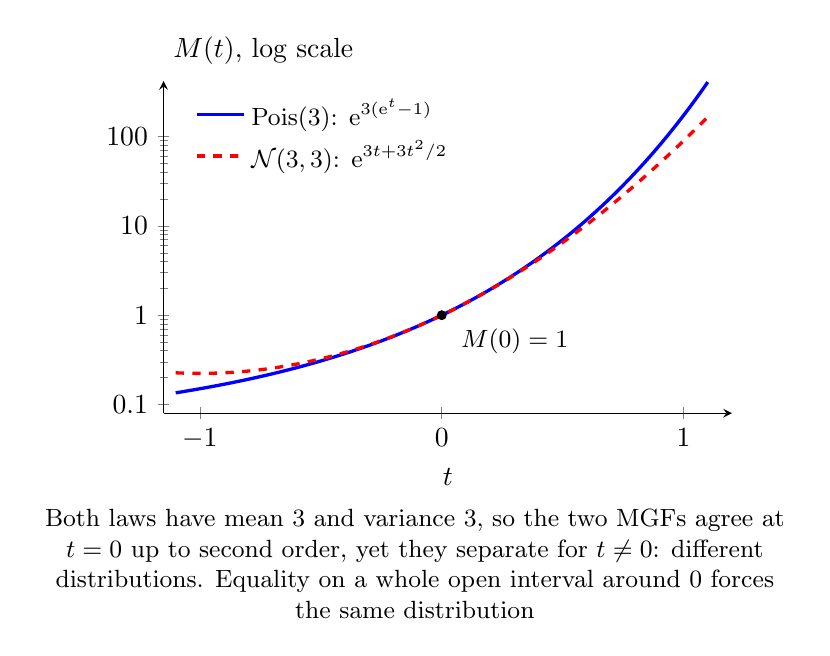
\begin{tikzpicture}
	\begin{axis}[
		axis lines=left, xmin=-1.15, xmax=1.2, ymin=0.08, ymax=420, ymode=log,
		xtick={-1,0,1}, ytick={0.1,1,10,100}, yticklabels={$0.1$,$1$,$10$,$100$},
		xlabel={$t$}, ylabel={$M(t)$, log scale}, ylabel style={rotate=-90, anchor=south west, at={(axis description cs:0,1.02)}},
		samples=120, smooth, width=8.8cm, height=5.8cm, clip=false,
		legend style={draw=none, fill=none, font=\small, at={(0.04,0.98)}, anchor=north west}, legend cell align=left
		]
		\addplot[blue, very thick, domain=-1.1:1.1] {exp(3*(exp(x)-1))};
		\addlegendentry{$\operatorname{Pois}(3)$: $\mathrm{e}^{3(\mathrm{e}^t-1)}$}
		\addplot[red, very thick, dashed, domain=-1.1:1.1] {exp(3*x+1.5*x^2)};
		\addlegendentry{$\mathcal{N}(3,3)$: $\mathrm{e}^{3t+3t^2/2}$}
		\fill[black] (axis cs:0,1) circle (1.8pt);
		\node[anchor=north west, font=\small] at (axis cs:0.04,0.9) {$M(0)=1$};
	\end{axis}
	\node[anchor=north, font=\small, align=flush center, text width=9.6cm] at ([yshift=-2pt]current axis.outer south) {Both laws have mean $3$ and variance $3$, so the two MGFs agree at $t=0$ up to second order, yet they separate for $t\ne0$: different distributions. Equality on a whole open interval around $0$ forces the same distribution};
\end{tikzpicture}
\end{document}
